% alt: Four horizontal bars, one above the other, each the chain of sites 1 to L divided into blocks of length t: the first bar reads P_1, dots, P_k in blue and then one grey segment R_k; in the second bar an orange segment R_{k+1} has appeared at the right end, at distance t+w from the start of R_k; in the third bar a blue block P_{k+1} has appeared inside the grey remainder, leaving two thin grey bands R_k of width w on either side of it; the fourth bar reads P_1, dots, P_k, P_{k+1} in blue and then R_{k+1} in orange, with the two thin bands gone.
% Section 10 (The sweep), Construction con:sweep (part2b_mps_protocol.tex): one step k of the sweep on the word P_1|...|P_k|R_k with a = kt+1 the first site of block k+1 and t = 20w (the bars are not to scale: w is drawn wider than t/20 so that the bands are visible). Row 1 is the word before step k; row 2 is after move (1), the birth of R_{k+1} on [a+t+w, L] inside R_k, so R_k keeps [a, a+t+w); row 3 is after move (2), the birth of P_{k+1} on [a+w, a+t-1] inside R_k, which leaves R_k the two bands [a, a+w-1] and [a+t, a+t+w-1]; row 4 is after moves (3) and (4), the dissolution of the two bands by Construction con:band (the first between C = P_k and B = P_{k+1}, the second between C = P_{k+1} and B = R_{k+1}), giving the word P_1|...|P_{k+1}|R_{k+1}. Ink-to-index: each bar is the chain Lambda = [1, L] with sites increasing to the right, each coloured segment is the set of sites owned by the party written in it (blue: a party P_i, grey: R_k, orange: R_{k+1}); the braces under the second bar mark the lengths t and w of the segments [a, a+t) and [a+t, a+t+w) kept by R_k; the labels above the bars are the site coordinates a = kt+1, a+w, a+t, a+t+w. No tensor is drawn and no leg is contracted.
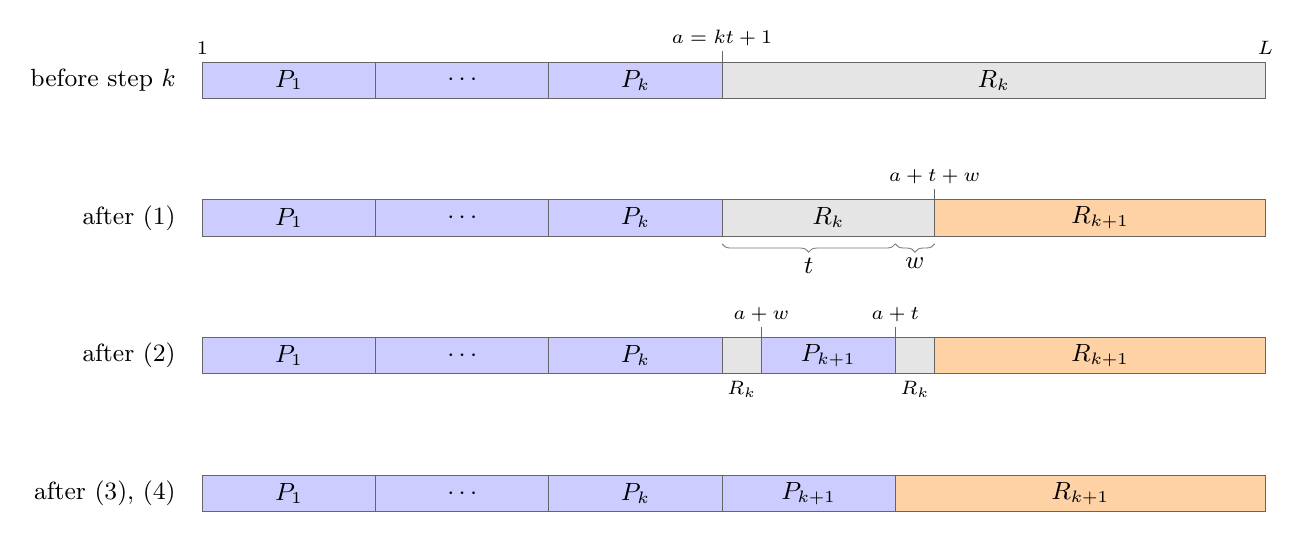
\begin{tikzpicture}[x=1cm, y=1cm, line width=0.3pt,
    lab/.style={font=\small, inner sep=1pt},
    name/.style={font=\scriptsize, text=black!55, inner sep=1pt},
    coord/.style={font=\scriptsize, inner sep=1pt},
    seg/.style={draw=black!60, line width=0.3pt},
    P/.style={seg, fill=blue!20},
    Rk/.style={seg, fill=black!10},
    Rn/.style={seg, fill=orange!35},
    brace/.style={decorate, decoration={brace, mirror, amplitude=3pt}}]
  % geometry: block length t, band width w (schematic, not t = 20 w), chain
  % from site 1 at x = 0 to site L at x = \L; the step is drawn for k = 3 with
  % the middle block standing for the blocks 2, ..., k-1
  \def\t{2.2}\def\w{0.5}\def\L{13.5}
  \def\a{6.6}      % a = k t + 1, the first site of block k+1 (3 t)
  \def\h{0.46}     % bar height
  \def\dy{1.75}    % row spacing
  % ---- row 1: before step k ----------------------------------------------
  \begin{scope}[yshift=0cm]
    \node[lab, anchor=east] at (-0.3, 0.5*\h) {before step \(k\)};
    \fill[P] (0, 0) rectangle (\t, \h);
    \fill[P] (\t, 0) rectangle (2*\t, \h);
    \fill[P] (2*\t, 0) rectangle (\a, \h);
    \fill[Rk] (\a, 0) rectangle (\L, \h);
    \node[lab] at (0.5*\t, 0.5*\h) {\(P_1\)};
    \node[lab] at (1.5*\t, 0.5*\h) {\(\cdots\)};
    \node[lab] at (2.5*\t, 0.5*\h) {\(P_k\)};
    \node[lab] at ({0.5*(\a+\L)}, 0.5*\h) {\(R_k\)};
    \node[coord, anchor=south] at (0, \h+0.05) {\(1\)};
    \node[coord, anchor=south] at (\L, \h+0.05) {\(L\)};
    \draw[black!60] (\a, \h) -- (\a, \h+0.14);
    \node[coord, anchor=south] at (\a, \h+0.16) {\(a=kt+1\)};
  \end{scope}
  % ---- row 2: after (1), birth of R_{k+1} on [a+t+w, L] -------------------
  \begin{scope}[yshift=-\dy cm]
    \node[lab, anchor=east] at (-0.3, 0.5*\h) {after (1)};
    \fill[P] (0, 0) rectangle (\t, \h);
    \fill[P] (\t, 0) rectangle (2*\t, \h);
    \fill[P] (2*\t, 0) rectangle (\a, \h);
    \fill[Rk] (\a, 0) rectangle (\a+\t+\w, \h);
    \fill[Rn] (\a+\t+\w, 0) rectangle (\L, \h);
    \node[lab] at (0.5*\t, 0.5*\h) {\(P_1\)};
    \node[lab] at (1.5*\t, 0.5*\h) {\(\cdots\)};
    \node[lab] at (2.5*\t, 0.5*\h) {\(P_k\)};
    \node[lab] at ({\a+0.5*(\t+\w)}, 0.5*\h) {\(R_k\)};
    \node[lab] at ({0.5*(\a+\t+\w+\L)}, 0.5*\h) {\(R_{k+1}\)};
    \draw[black!60] (\a+\t+\w, \h) -- (\a+\t+\w, \h+0.14);
    \node[coord, anchor=south] at (\a+\t+\w, \h+0.16) {\(a+t+w\)};
    \draw[brace, black!55] (\a, -0.1) -- (\a+\t, -0.1)
      node[lab, midway, below=4pt, text=black] {\(t\)};
    \draw[brace, black!55] (\a+\t, -0.1) -- (\a+\t+\w, -0.1)
      node[lab, midway, below=4pt, text=black] {\(w\)};
  \end{scope}
  % ---- row 3: after (2), birth of P_{k+1} on [a+w, a+t-1] -----------------
  \begin{scope}[yshift=-2*\dy cm]
    \node[lab, anchor=east] at (-0.3, 0.5*\h) {after (2)};
    \fill[P] (0, 0) rectangle (\t, \h);
    \fill[P] (\t, 0) rectangle (2*\t, \h);
    \fill[P] (2*\t, 0) rectangle (\a, \h);
    \fill[Rk] (\a, 0) rectangle (\a+\w, \h);
    \fill[P] (\a+\w, 0) rectangle (\a+\t, \h);
    \fill[Rk] (\a+\t, 0) rectangle (\a+\t+\w, \h);
    \fill[Rn] (\a+\t+\w, 0) rectangle (\L, \h);
    \node[lab] at (0.5*\t, 0.5*\h) {\(P_1\)};
    \node[lab] at (1.5*\t, 0.5*\h) {\(\cdots\)};
    \node[lab] at (2.5*\t, 0.5*\h) {\(P_k\)};
    \node[lab] at ({\a+0.5*(\t+\w)}, 0.5*\h) {\(P_{k+1}\)};
    \node[lab] at ({0.5*(\a+\t+\w+\L)}, 0.5*\h) {\(R_{k+1}\)};
    \node[coord, anchor=north] at (\a+0.5*\w, -0.06) {\(R_k\)};
    \node[coord, anchor=north] at (\a+\t+0.5*\w, -0.06) {\(R_k\)};
    \draw[black!60] (\a+\w, \h) -- (\a+\w, \h+0.14);
    \node[coord, anchor=south] at (\a+\w, \h+0.16) {\(a+w\)};
    \draw[black!60] (\a+\t, \h) -- (\a+\t, \h+0.14);
    \node[coord, anchor=south] at (\a+\t, \h+0.16) {\(a+t\)};
  \end{scope}
  % ---- row 4: after (3), (4), the two bands dissolved ---------------------
  \begin{scope}[yshift=-3*\dy cm]
    \node[lab, anchor=east] at (-0.3, 0.5*\h) {after (3), (4)};
    \fill[P] (0, 0) rectangle (\t, \h);
    \fill[P] (\t, 0) rectangle (2*\t, \h);
    \fill[P] (2*\t, 0) rectangle (\a, \h);
    \fill[P] (\a, 0) rectangle (\a+\t, \h);
    \fill[Rn] (\a+\t, 0) rectangle (\L, \h);
    \node[lab] at (0.5*\t, 0.5*\h) {\(P_1\)};
    \node[lab] at (1.5*\t, 0.5*\h) {\(\cdots\)};
    \node[lab] at (2.5*\t, 0.5*\h) {\(P_k\)};
    \node[lab] at (\a+0.5*\t, 0.5*\h) {\(P_{k+1}\)};
    \node[lab] at ({0.5*(\a+\t+\L)}, 0.5*\h) {\(R_{k+1}\)};
  \end{scope}
\end{tikzpicture}
